% !TeX spellcheck = de_DE
\documentclass{beamer}
\usepackage[utf8]{inputenc}
\usepackage[T1]{fontenc}
\usepackage[ngerman]{babel}
\usepackage{graphicx}
\usepackage{gensymb}
\usepackage{bold-extra}
\usepackage{textcomp}
\usepackage{csquotes}
\usepackage{soul}
\usepackage{fancyvrb}

\input{../flat-blue-theme.inc}
\input{../footnotes.inc}

\setcounter{tocdepth}{1}

\setbeamercovered{invisible}
\beamertemplatenavigationsymbolsempty
\renewcommand*\insertshorttitle
{
	% To not count \pause as new frame. And also to make the package "appendixnumberbeamer" work.
	\makebox[0.94\textwidth]{\oldmacro\hfill\insertframenumber\,/\,\inserttotalframenumber}
}
\condensedToc

\title{OpenStreetMap}
\subtitle{Offene Geodaten und wie man beitragen kann}
\author[Hauke Stieler -- 4stieler@inf]{Hauke Stieler\\4stieler@inf}
\titlegraphic{
\includegraphics[width=1.5cm]{images/openstreetmap-logo.png}}
%\date{\today}
\date{24. Januar 2024}

\begin{document}
	{
		\setbeamertemplate{footline}{}
		\setbeamertemplate{headline}{}
		\maketitle
		\addtocounter{page}{-1}
	}
	
	\begin{frame}{Über mich}
		\begin{itemize}
			\item Hauke
			\item SSE + Inf Master
			\pause
			\item Open Source / Open Data interessiert
			\item Softwareentwickler (viel mit Geo-Zeugs)
			\pause
			\item OSMler seit 13.04.2019 (Nutzername \enquote{hauke-stieler})
			\begin{itemize}
				\item 5.478 Änderungssätze
				\item 472.462 Änderungen
				\item Fokus auf Radinfrastruktur, Outdoor, POIs
				\item OSMF Mitglied
			\end{itemize}
		\end{itemize}
	\end{frame}
	
	\begin{frame}
		\tableofcontents
	\end{frame}
	
	\section{Geodaten Grundlagen}
	
		\subsection{Geodaten Grundlagen}
	
		\begin{frame}{Was sind \enquote{Geodaten}?}
			\begin{definition}
				Informationen/Daten mit geografischem Bezug.
			\end{definition}
			\begin{itemize}
				\item Haus mir Adresse\pause
				\item Messdaten mit Koordinate\pause
				\item Luftbilder\pause
				\item aufgenommener GPX-track\pause
				\item ...
			\end{itemize}
		\end{frame}
		
		\begin{frame}{Formate}
			\begin{columns}[t]
				\begin{column}{0.47\textwidth}
					Vektorformate
					\begin{itemize}
						\item GeoJSON
						\item GeoPackage, SpatiaLite
						\item Shapefile
						\item KML, GML, WKT, OSM
					\end{itemize}
					\pause
					Rasterformate
					\begin{itemize}
						\item GeoTIFF
						\item netCDF, JPEG2000
					\end{itemize}
					\pause
				\end{column}
				\begin{column}{0.53\textwidth}
					Datenbank:
					\begin{itemize}
						\item SQlite \textrightarrow\ GeoPackage, SpatiaLite
						\item Postgres + PostGIS
					\end{itemize}
					\pause
					Webstandards:
					\begin{itemize}
						\item OGC (WMS, WFS, ...)
						\item XYZ-tiles
						\item ArcGIS
					\end{itemize}
				\end{column}
			\end{columns}
		\end{frame}
		
		\begin{frame}{Vaktordaten (GeoJSON)}
			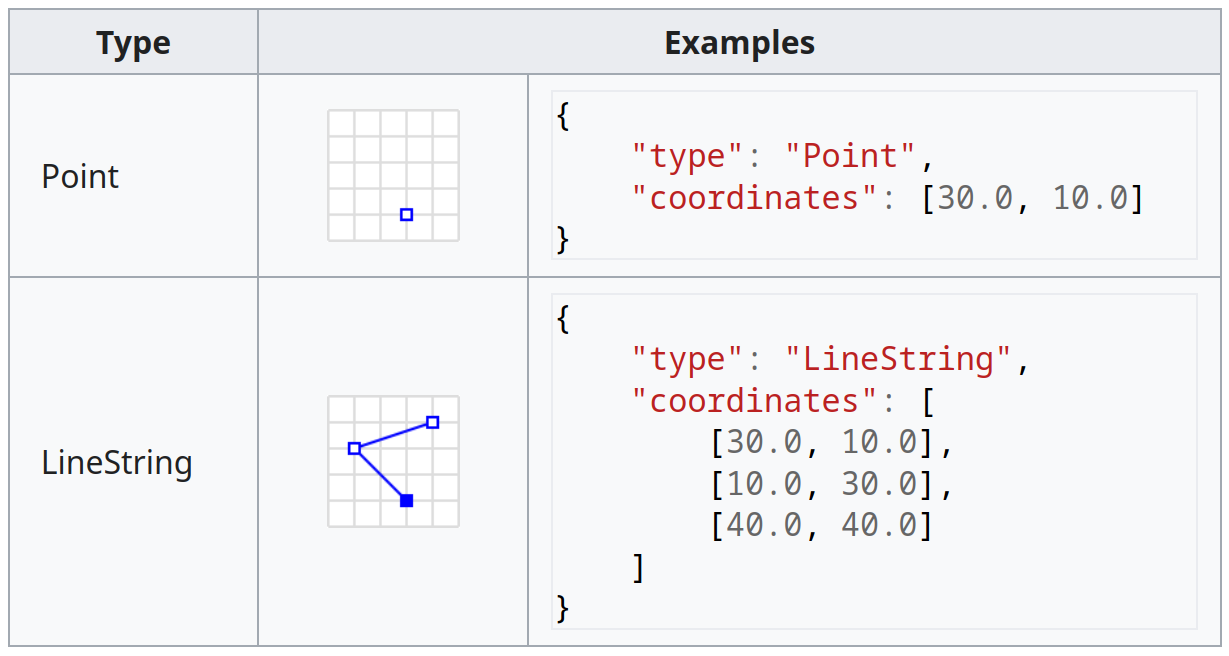
\includegraphics[width=\textwidth]{images/geodata-vector-1.png}\footnote{\href{https://en.wikipedia.org/wiki/GeoJSON}{Wikipedia -- GeoJSON}}
		\end{frame}
		
		\begin{frame}{Vaktordaten (GeoJSON)}
			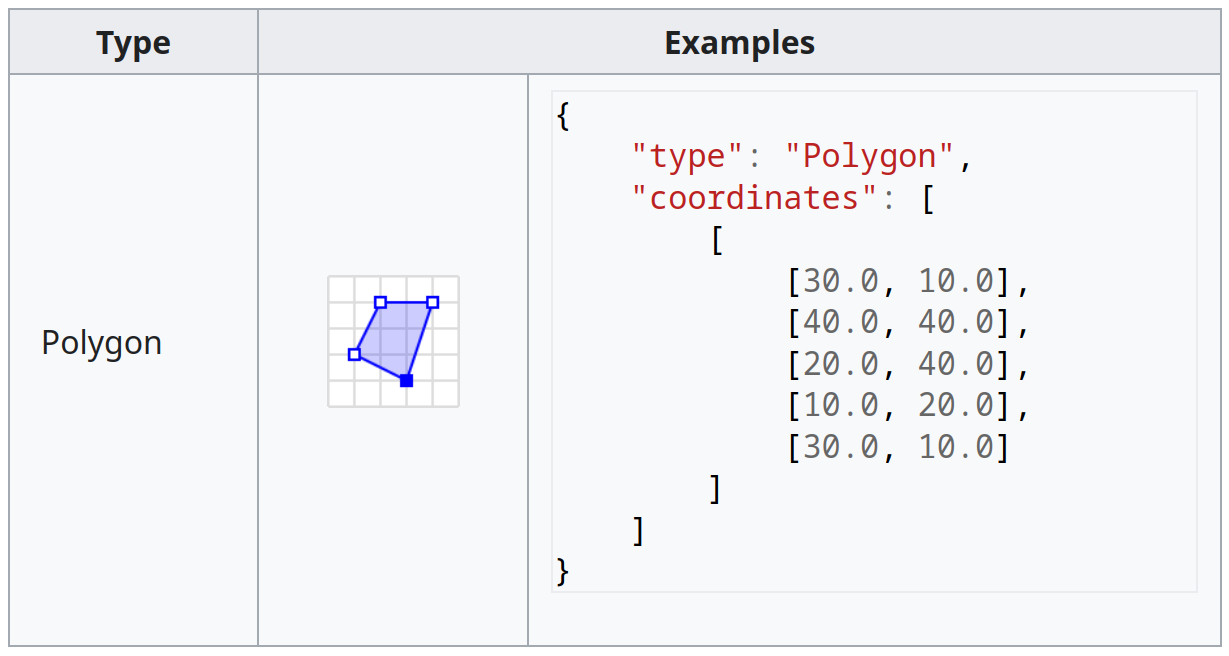
\includegraphics[width=\textwidth]{images/geodata-vector-2.png}\footnote{\href{https://en.wikipedia.org/wiki/GeoJSON}{Wikipedia -- GeoJSON}}
		\end{frame}
		
		\begin{frame}{Attribute}
			\begin{itemize}
				\item auch: Eigenschaften / Felder / Properties
				\item ergänzende Infos an Daten
				\begin{itemize}
					\item Geometrie: \textit{Wo} ist es?
					\item Attribute: \textit{Was} ist es?
				\end{itemize}\pause
				\item einfache Key-Value Paare\pause
				\item Formate definieren ggf. Wertebereiche und Typen
			\end{itemize}
			\pause
			\vspace{0.25cm}
			\begin{center}
				Geometrie + Attribute = \enquote{Feature}
			\end{center}
		\end{frame}
		
	\section{OSM Überblick}
	
		\begin{frame}
			\tableofcontents[currentsection]
		\end{frame}

		\subsection{Was ist OSM?}
	
			\begin{frame}{Was ist OSM?}
				\begin{itemize}
					\item Projekt zum Sammeln und Bereitstellen freier\footnote{\textit{free} as in \textit{free}dom} Geodaten
					\item offene Datenbank unter ODbL (Open Database License)\pause
					\item finanziert durch Spenden, Konferenzen, Mitgliedschaften
					\item OpenStreetMap Foundation (OSMF)\pause
					\item Geschichte
					\begin{itemize}
						\item 2004 -- Projekt in Englang gestartet
						\item 2006 -- OSMF registriert
						\item 2009 -- Release aktueller API Version
						\item 2013 -- 1 Mio. registrierte Nutzer
						\item 2024 -- Ca. 11 Mio. registrierte Nutzer
					\end{itemize}
				\end{itemize}
			\end{frame}
			
			\begin{frame}{Statistiken}
				\begin{itemize}
					\item 435k EUR Einnahmen in 2022
					\item 11 Mio. Beitragende (\enquote{contributors})
					\item 40k monatliche / 250-300k jährliche contributor
					\item 110 Mio. Änderungen pro Monat\footnote{Oder 42/s; 2750 edits pro contributor pro Monat}
					\item 8,8 Mrd. Punkt / 1 Mrd. Linien/Polygone / 11 Mio. Relationen
					\item Tile server: 50.000 requests/Min.
				\end{itemize}
			\end{frame}

			\begin{frame}{Warum OSM?}
				\begin{columns}[t]
					\begin{column}{0.5\textwidth}
						Proprietäre Karten\pause
						\begin{itemize}
							\item oft veraltet und fehlerhaft\pause
							\item kein Beitragen möglich\pause
							\item kein Zugriff die Rohdaten\pause
							\item Fokus auf Autos und Verkehr\pause
							\item Lizenzprobleme noch und nöcher
						\end{itemize}
					\end{column}
					\pause
					\begin{column}{0.5\textwidth}
						Amtliche/offizielle Daten\pause
						\begin{itemize}
							\item oft veraltet und fehlerhaft\pause
							\item kein Beitragen möglich\pause
							\item nicht immer Zugriff die Rohdaten\pause
							\item nicht für allgemeine Anwendungsfälle gemacht (z.B. Routing)
						\end{itemize}
						\pause
						Aber:\\
						Es tut sich was, mehr und mehr Daten werden frei veröffentlicht.
					\end{column}
				\end{columns}
			\end{frame}
			
			\begin{frame}{Zeug bereitgestellt durch die OSMF}
				\begin{itemize}
					\item Datenbank, Backup-Server, Mirror
					\item API Server
					\item Tile rendering (nahezu in Echtzeit!)
					\pause
					\item Geocoder\footnote{Suche nach Orten}, mehrere Routing-Engines
					\item Overpass (Query-Tool)
					\pause
					\item Interne Dienste
					\begin{itemize}
						\item Statistiken über die Daten (taginfo)
						\item Wiki
						\item git, trac, irc, BBB, ......
					\end{itemize}
				\end{itemize}
				\pause
				\textrightarrow\ \href{https://hardware.openstreetmap.org/}{hardware.osm.org}
			\end{frame}
			
			\begin{frame}{Zeug bereitgestellt durch andere}
				\begin{itemize}
					\item Karten und Kartenstile
					\begin{itemize}
						\item \href{https://map.openseamap.org/?zoom=13.5\&lon=9.96566\&lat=53.52952}{OpenSeaMap}
						\item \href{https://opentopomap.org}{OpenTopoMap}
						\item standard \href{https://github.com/gravitystorm/openstreetmap-carto}{OSM-Carto} Stil
					\end{itemize}
					\pause
					\item Mirror- und Dienste zum Daten runterladen
					\pause
					\item Online-Dienste: \href{https://print.get-map.org/}{MyOSMatic}, \href{https://maps.openrouteservice.org}{ORS}, \href{https://umap.openstreetmap.de}{uMap}
					\pause
					\item Apps, Tools, Frameworks, Bibliotheken, etc.
				\end{itemize}
				\pause
				\vspace{0.5cm}
				Und noch viel mehr \textrightarrow\ \href{https://wiki.openstreetmap.org/wiki/List\_of\_OSM-based\_services}{OSM-Wiki: List of OSM-based services}
			\end{frame}
			
			\begin{frame}{Beispiel: OpenRouteService (ORS)}
				\begin{center}
					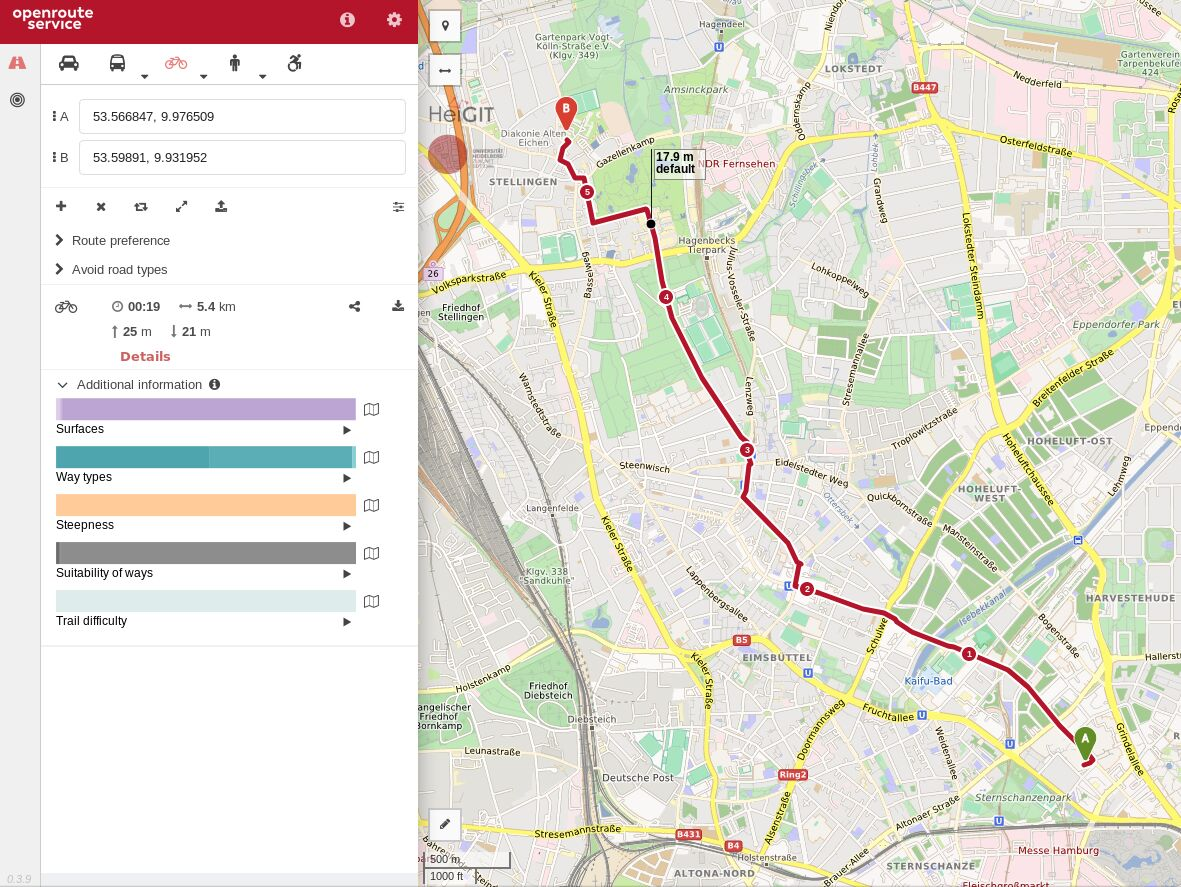
\includegraphics[height=0.7\textheight]{images/openrouteservice.jpg}\\
					\url{https://maps.openrouteservice.org}
				\end{center}
			\end{frame}
			
			\begin{frame}{Beispiel: Wheelmap}
				\begin{center}
					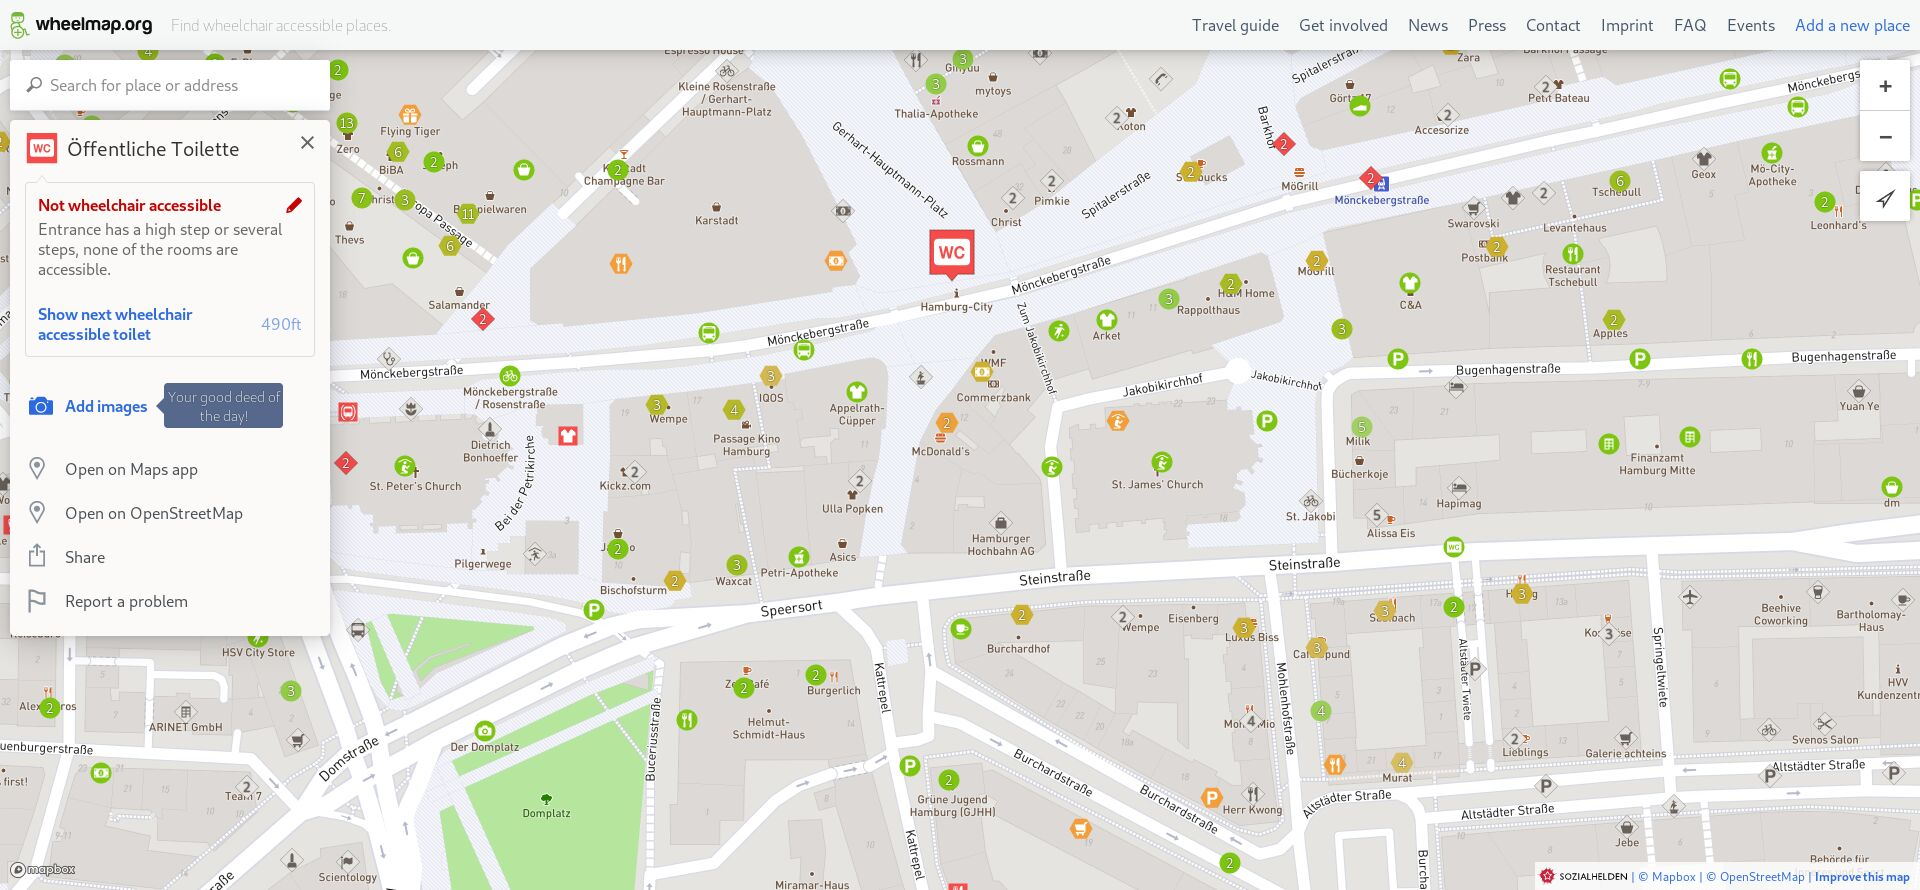
\includegraphics[height=0.7\textheight]{images/wheelmap-website.jpg}\\
					\url{https://wheelmap.org}
				\end{center}
			\end{frame}

		\subsection{Community}
		
			\begin{frame}{Was macht die so?}
				\begin{itemize}
					\item Daten beitragen (\enquote{mapping})
					\begin{itemize}
						\item raus gehen und Daten sammeln
						\item externe Quellen anzapfen (z.B. Luftbilder)
					\end{itemize}\pause
					\item Software und Tools entwickeln\pause
					\item Dokumentation erstellen und pflegen\pause
					\item Events organisieren (Konferenzen, Mapathons, Workshops, Stammtische, ...)\pause
					\item mit nicht-mappern reden (z.B. in Schulden, Geschäften, Ämtern, ...)
				\end{itemize}
			\end{frame}
		
			\begin{frame}{Organisation der Community}
				\begin{itemize}
					\item \href{https://wiki.openstreetmap.org/}{Wiki}
					\item \href{https://wiki.openstreetmap.org/wiki/Mailing_lists}{Mailinglisten}
					\item \href{https://community.openstreetmap.org/}{Forum}
					\item \href{https://wiki.openstreetmap.org/wiki/Contact_channels}{Weiteres}: Discord, Telegram, Mastodon, Reddit, ...)
				\end{itemize}
			\end{frame}

	\section{OSM Daten}
		
		\begin{frame}
			\tableofcontents[currentsection]
		\end{frame}
		
		\subsection{Tags (Attribute)}
		
			\begin{frame}
				\begin{itemize}
					\item Key-Value Paare (untypisiert)
					\item standardisiert durch Community-Proposals
					\item zentrale Doku (\enquote{die Wahrheit}): Wiki
					\item trotzdem: freies Tagging-System
				\end{itemize}
			\end{frame}
		
		\subsection{Geometrien}
		
			\begin{frame}[fragile]{Node (Punkt)}
				\begin{center}
					\begin{columns}
						\begin{column}{1.25cm}
							\centering
							
\includegraphics[width=1cm]{images/240px-Mf_node.png}
						\end{column}
						\begin{column}{3.75cm}
							\centering
							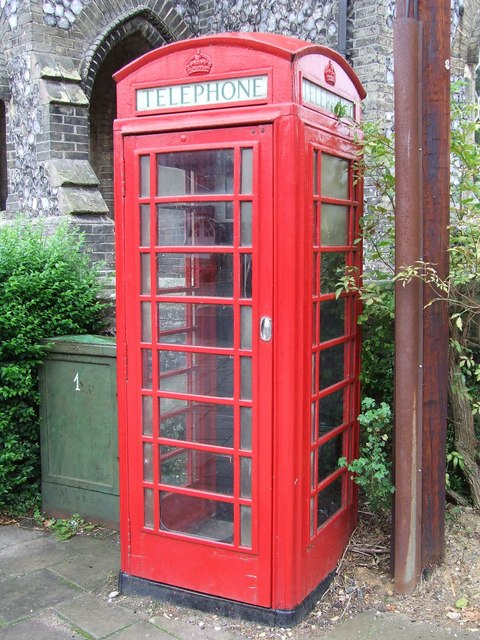
\includegraphics[width=3.5cm]{images/red-telephone-box-uk.jpg}\\
							\textcolor{gray}{
								\tiny
								\href{https://wiki.openstreetmap.org/wiki/File:Red\_telephone\_box\_-\_geograph.org.uk\_-_919348.jpg}{OSM-wiki}
							}
						\end{column}
						\begin{column}{3.5cm}
							\begin{verbatim}
								amenity=telephone
								covered=booth
							\end{verbatim}
							\begin{center}
								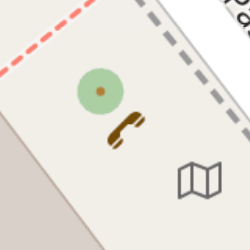
\includegraphics[height=3cm]{images/telephone.png}
							\end{center}
						\end{column}
					\end{columns}
				\end{center}
			\end{frame}
		
			\begin{frame}[fragile]{Way (Linien)}
				\begin{center}
					\begin{columns}
						\begin{column}{1cm}
							\centering
							
\includegraphics[width=1cm]{images/240px-Mf_way.png}
						\end{column}
						\begin{column}{4.5cm}
							\centering
							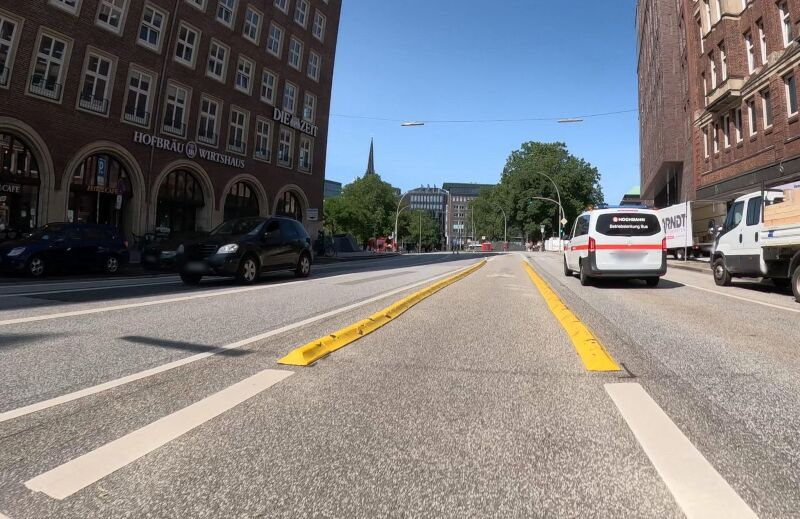
\includegraphics[width=4.5cm]{images/way-example.jpg}
							\textcolor{gray}{
								\tiny
								\href{https://www.mapillary.com/app/?pKey=680503257254203}{Mapillary}
							}
						\end{column}
						\begin{column}{3.5cm}
							\begin{verbatim}
								highway=secondary
								oneway=yes
								name=Speersort
							\end{verbatim}
							\begin{center}
								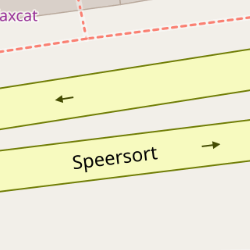
\includegraphics[height=3cm]{images/secondary.png}
							\end{center}
						\end{column}
					\end{columns}
				\end{center}
			\end{frame}
			
			\begin{frame}[fragile]{Area (Polygon = geschlossener Way)}
				\begin{center}
					\begin{columns}
						\begin{column}{1cm}
							\centering
							
\includegraphics[width=1cm]{images/240px-Mf_area.png}
						\end{column}
						\begin{column}{4.5cm}
							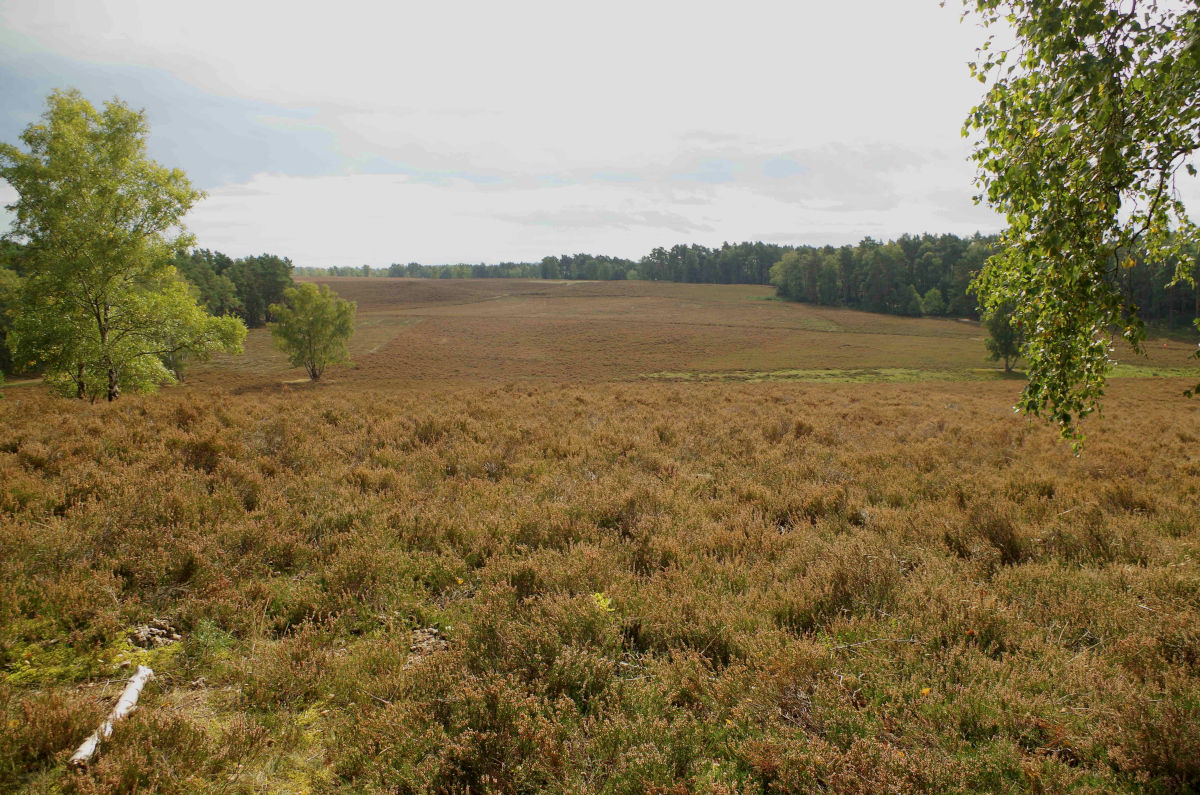
\includegraphics[width=4.5cm]{images/area-example.jpg}
						\end{column}
						\begin{column}{4cm}
							\begin{verbatim}
								natural=heath
								name=Fischbeker Heide
							\end{verbatim}
							\begin{center}
								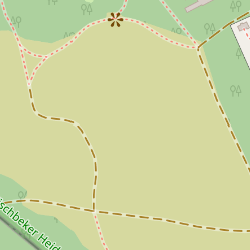
\includegraphics[height=3cm]{images/heath.png}
							\end{center}
						\end{column}
					\end{columns}
				\end{center}
			\end{frame}
	
			\begin{frame}[fragile]{Relation: Zusammenschluss mehrerer Features}
				\begin{center}
					\begin{columns}
						\begin{column}{1.25cm}
							\centering
							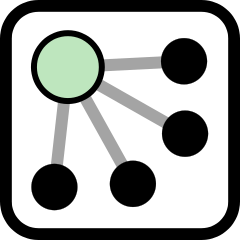
\includegraphics[width=1cm]{images/240px-Mf_relation.png}
						\end{column}
						\begin{column}{4cm}
							\begin{verbatim}
								type=route
								route=bus
								ref=4
							\end{verbatim}
							\vspace{0.25cm}
							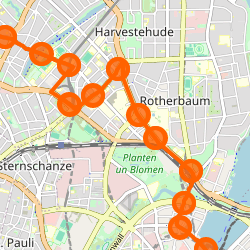
\includegraphics[width=3.75cm]{images/relation-example.png}
						\end{column}
						\begin{column}{4cm}
							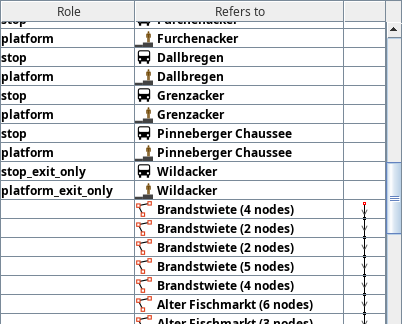
\includegraphics[width=4cm]{images/relation-list.png}
						\end{column}
					\end{columns}
				\end{center}
			\end{frame}
			
			\begin{frame}{Multipolygon (Relation; Polygon in Polygon)}
				\begin{center}
					\texttt{farmland=center}
					\vspace{0.5cm}
					\begin{columns}
						\begin{column}{4cm}
							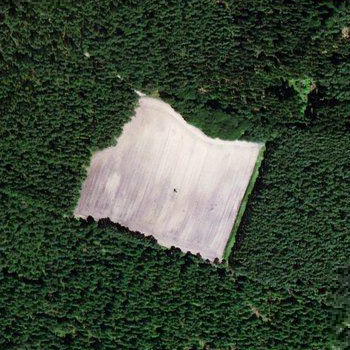
\includegraphics[width=\linewidth]{images/multipolygon-example.png}
						\end{column}
						\begin{column}{4cm}
							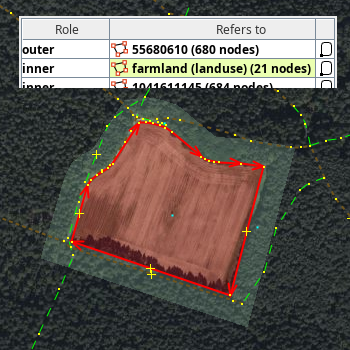
\includegraphics[width=\linewidth]{images/multipolygon-josm.png}
						\end{column}
					\end{columns}
					\vspace{0.25cm}
					\textcolor{gray}{\tiny Imagery: Microsoft\copyright Bing(tm) Maps Platform}
				\end{center}
			\end{frame}
			
			\begin{frame}[fragile]{OSM-XML Format}
				OSM nutzt ein XML Format (\texttt{.osm}; oft komprimiert in eine \texttt{.osm.pbf} Datei):
				\vspace{0.25cm}
				{
					\scriptsize
					\begin{Verbatim}
<?xml version='1.0' encoding='UTF-8'?>
<osm version='0.6' generator='JOSM'>
    <node id='1' action='modify' visible='true' lat='53.558' lon='9.991' />
    <node id='2' action='modify' visible='true' lat='53.548' lon='9.972' />
    <node id='3' action='modify' visible='true' lat='53.545' lon='9.997' />
    <way id='4' action='modify' visible='true'>
        <nd ref='1' />
        <nd ref='2' />
        <nd ref='3' />
        <tag k='highway' v='tertiary' />
        <tag k='name' v='Vogt-Kölln-Straße' />
    </way>
</osm>
					\end{Verbatim}
				}
			\end{frame}
			
		\subsection{Daten in OSM}
			
			\begin{frame}{Welche Daten sind in OSM?}
				Alle möglichen öffentlich zugängliche Dinge
				\begin{itemize}
					\item Bauwerke, Straßen und Wege
					\item POIs (Restaurants, Museen, Hydranten, ...)
					\item Infrastruktur (Parkplätze, Stromleitungen, Gleise, ...)
					\item Landschaftsformen (Wälder, Seen, Grünflächen, ...)
					\item Routen (Busrouten, Wanderwege, MTB-Trails, ...)
					\item .........
				\end{itemize}
				\pause
				Nicht (immer) enthalten:
				\begin{itemize}
					\item privates, personenbezogenes, nicht freigegebenes
					\item nicht verifizierbares
				\end{itemize}
				\pause
				Mehr Details im Wiki \textrightarrow\ \href{https://wiki.openstreetmap.org/wiki/Map\_features}{Map features}
			\end{frame}
			
	\section{Die Daten nutzen}
			
		\begin{frame}
			\tableofcontents[currentsection]
		\end{frame}
		
		\subsection{Die Daten nutzen}
			
			\begin{frame}{Nutzungsbedingungen}
				Man kann einfach ...
				\begin{itemize}
					\item[...] Daten runterladen.
					\item[...] Daten für private und kommerzielle Zwecke nutzen.
					\item[...] Daten weitergeben, gilt auch für abgeleitete Werte (\enquote{derivative works}; z.B. gedruckte Karten).
				\end{itemize}
				\pause
				\vspace{0.25cm}
				\textbf{Aber} unter Beachtung der ODbL:
				\begin{itemize}
					\item \href{https://osmfoundation.org/wiki/Licence/Attribution\_Guidelines}{Attribution}!
					\item Weitergabe unter ODbL
				\end{itemize}
			\end{frame}
			
			\begin{frame}{Auf Daten zugreifen}
				\begin{itemize}
					\item für kleine Gebiete
					\begin{itemize}
						\item osm.org \textrightarrow\ \enquote{Export} \textrightarrow\ Gebiet auswählen \textrightarrow\ \enquote{Export}
						\item API: \href{https://www.openstreetmap.org/api/0.6/map?bbox=9.93116,53.59846,9.93572,53.60052}{\texttt{osm.org/api/0.6/map?bbox=...}}
						\item \href{https://overpass-turbo.eu/}{Overpass API} (Filterung + Download verschiedener Formaten)
					\end{itemize}\pause
					\item für große Gebiete
					\begin{itemize}
						\item \href{https://download.geofabrik.de/}{Geofabrik GmbH}
						\item Alles (\texttt{planet.osm} Dump; wöchentlich aktualisiert; >70GB OSM-PBF Datei)
					\end{itemize}
				\end{itemize}
			\end{frame}
			
			\begin{frame}{Daten verarbeiten/nutzen}
				Libraries, Frameworks:
				\begin{itemize}
					\item GDAL, GeoTools: Schweizer Taschenmesser für Geodaten
					\item libosmium: OSM-spezifische C-Library (Python- \& Node-bindings)
					\item Leaflet/OpenLayers/MapLibre: Daten auf Karte anzeigen
				\end{itemize}
				\pause
				CLI Tools:
				\begin{itemize}
					\item ogr2ogr: Teil von GDAL zum konvertieren von Daten
					\item osmium: Generisches Tool für OSM-Daten
					\item osmosis: Ähnlich zu osmium, aber eher deprecated
					\item osm2pgsql: OSM-Daten in PostgreSQL-Datenbank importieren
				\end{itemize}
			\end{frame}
		
			\begin{frame}{Daten verarbeiten/nutzen}
				Desktop Anwendungen:
				\begin{itemize}
					\item QGIS: \textit{Die} Open-Source GIS-Anwendung
					\item JOSM: OSM-Editor, nützlich für simple Verarbeitungen
				\end{itemize}
				\pause
				DB, Server und hosting:
				\begin{itemize}
					\item Geoserver, Mapserver
					\item PostgreSQL + PostGIS
					\item Tilemaker, tileserver-gl, Maputnik
					\item Mapnik, Carto, TileMill
				\end{itemize}
				\pause
				\vspace{0.25cm}
				Mehr dazu im Wiki \textrightarrow\ \href{https://wiki.openstreetmap.org/wiki/Software}{Software}
			\end{frame}

	\section{Zu OSM beitragen}
	
		\begin{frame}
			\tableofcontents[currentsection]
		\end{frame}
		
		\subsection{Zu OSM beitragen}
		
			\begin{frame}{Ablauf einer Bearbeitung (Überblick)}
				\begin{enumerate}
					\item registrieren auf \href{https://www.openstreetmap.org/user/new}{osm.org}\pause
					\item für einen Editor entscheiden
					\begin{itemize}
						\item Web: iD
						\item Desktop: JOSM
						\item Mobil: StreetComplete, OsmAnd, Vespucci
					\end{itemize}\pause
					\item Änderungen machen\pause
					\item Änderungen hochladen (\enquote{changeset}\footnote{Ähnlich zu einem Commit bei git.} erstellen)
				\end{enumerate}
			\end{frame}
			
			\begin{frame}{Editoren: iD}
				\begin{center}
					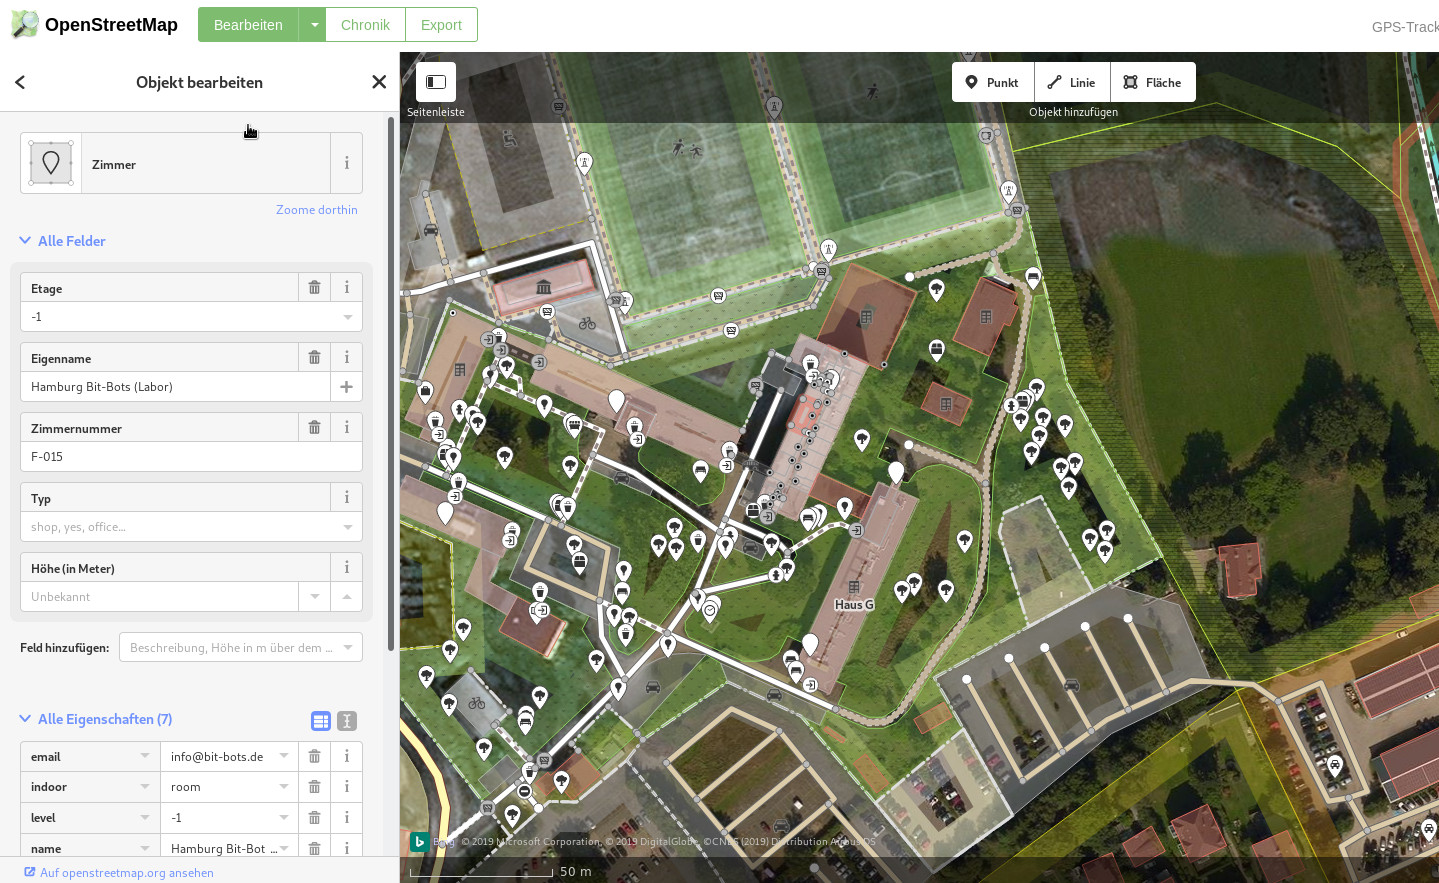
\includegraphics[height=0.75\textheight]{images/id-editor.jpg}
					\href{https://www.openstreetmap.org/edit}{osm.org/edit}
				\end{center}
			\end{frame}
			
			\begin{frame}{Editoren: JOSM}
				\begin{center}
					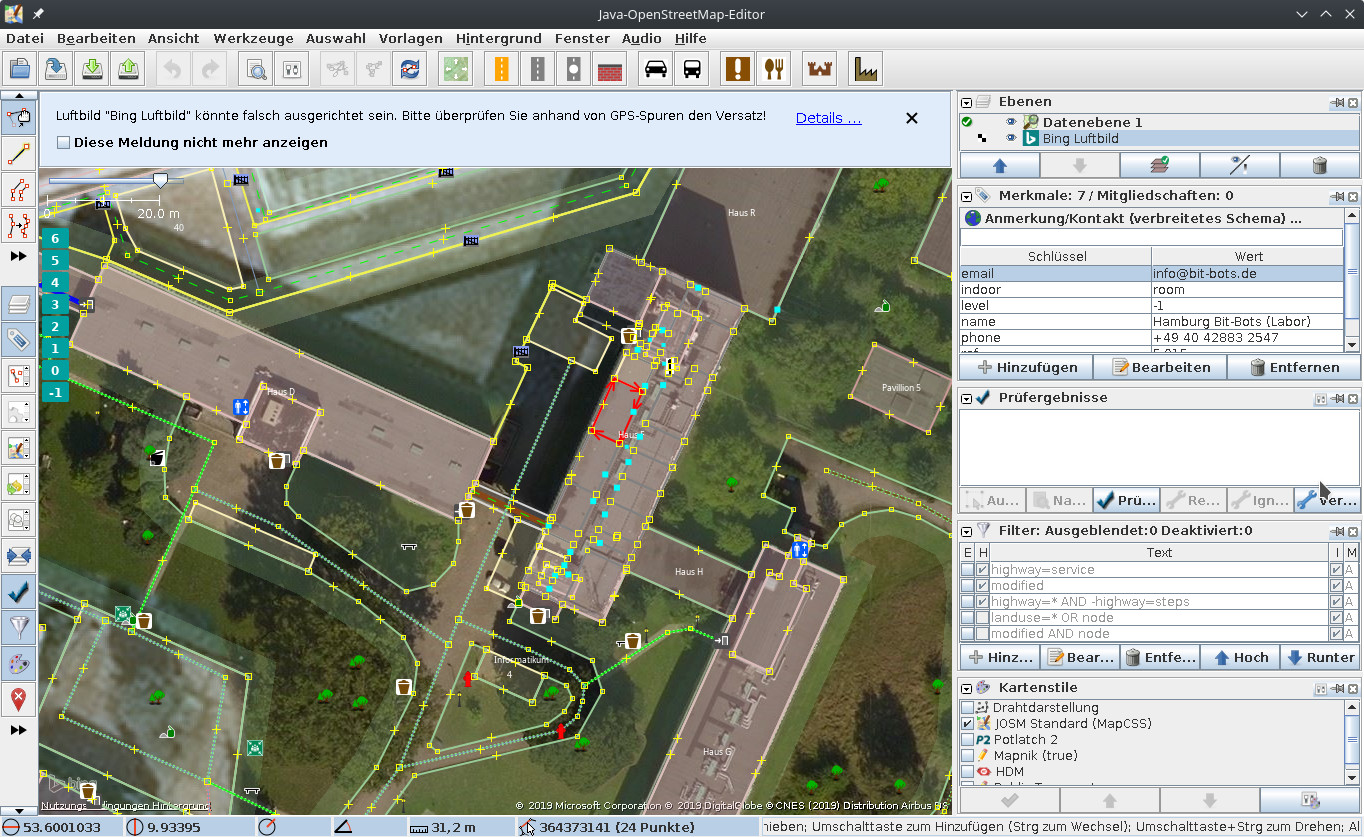
\includegraphics[height=0.75\textheight]{images/josm-editor.jpg}
					\href{https://josm.openstreetmap.de/}{josm.osm.org}
				\end{center}
			\end{frame}
			
			\begin{frame}{Änderungen machen}
				Bevor es los geht: Daten sammeln (z.B. beim Wandern)
				\begin{itemize}
					\item Notizen oder Photos machen
					\item GPS-Tracks aufnehmen
				\end{itemize}
				\pause
				\vspace{0.25cm}
				Ablauf in iD und JOSM:
				\begin{enumerate}
					\item Editor öffnen und Rohdaten laden\pause
					\item mit nötigen Tags vertraut machen \textrightarrow\ Wiki\pause
					\item ergänze/ändere/lösche Daten
				\end{enumerate}
			\end{frame}
			
			\begin{frame}{Änderungen hochladen}
				Ablauf in iD und JOSM:
				\begin{enumerate}
					\item eigene Änderungen reviewen\pause
					\item den \enquote{Hochladen}/\enquote{Speichern} Button klicken\pause
					\item Textfelder ausfüllen:
					\begin{itemize}
						\item Kommentar/comment: Kurze Beschreibung der Änderungen
						\item Quellen/source: Ursprung der Daten (siehe \href{https://wiki.openstreetmap.org/wiki/Key:source}{Wiki} für Infos dazu)
					\end{itemize}\pause
					\item auf \enquote{Hochladen} klicken
				\end{enumerate}
				\pause
				\vspace{0.25cm}
				{
					\setbeamercolor{block title}{bg=orange!65, fg=black}
					\setbeamercolor{block body}{bg=orange!25}
					\begin{block}{Wichtig!}
						Hochgeladener \enquote{changeset} ist \textbf{sofort} live in der Produktivdatenbank, daher sorgfältig arbeiten!
					\end{block}
				}
			\end{frame}
			
			\begin{frame}{Exkurs: Externe Quellen nutzen}
				Beispiel:
				\begin{itemize}
					\item Luftbilder (z.B. ESRI World Imagery)
					\item amtliche Daten (z.B. ALKIS\footnote{Amtliches Liegenschaftskatasterinformationssystem})
					\item Fotos, Zeitungsartikel, Lagepläne, amtliche Bekanntmachungen, Websites, etc.
				\end{itemize}
				\pause
				\vspace{0.25cm}
				{
					\setbeamercolor{block title}{bg=orange!65, fg=black}
					\setbeamercolor{block body}{bg=orange!25}
					\begin{block}{Wichtig!}
						Lizenzen \textbf{müssen} immer \href{https://wiki.openstreetmap.org/wiki/Import/ODbL_Compatibility}{kompatibel mit OSM sein}! Ggf. Urheber kontaktieren und Genehmigung einholen!
					\end{block}
				}
			\end{frame}
			
			\begin{frame}{Exkursion: Open Data in Deutschland}
				Wohin geht die Reise?
				\begin{itemize}
					\item Rechtliche Öffnung der Daten
					\begin{itemize}
						\item Lizenz häufig: CC BY-SA 4.0, DL-DE BY 2.0, CC0
					\end{itemize}\pause
					\item Technische Öffnung der Daten
					\begin{itemize}
						\item web APIs (OGC-konform)
						\item professionelle Formate (kein \texttt{.pdf}, \texttt{.csv} oder \texttt{.xlsx} WTF?!)
					\end{itemize}
				\end{itemize}
				\pause
				\vspace{0.25cm}
				Zugriff via APIs/Websites, z.B. \href{https://www.geoportal.de/}{geoportal.de}.
			\end{frame}
			
			\begin{frame}{Andere Möglichkeiten beizutragen}
				\begin{itemize}
					\item fehlerhafte/unvollständige/fehlende Daten melden
					\begin{enumerate}
						\item auf osm.org gehen
						\item Rechtsklick auf Karte \textrightarrow\ \enquote{Add a note here}
						\item nützliche Infos ergänzen (so viele Infos wie möglich)
						\item wichtig: Man brauchen einen Account zum Antworten auf Rückfragen
					\end{enumerate}\pause
					\item mit Unternehmen/Ämtern sprechen um Genehmigungen zu bekommen\pause
					\item Events organisieren\pause
					\item allgemein Werbung machen (spread the word)
				\end{itemize}
			\end{frame}
			
		\subsection{}
			
			\begin{frame}
				\begin{center}
					
\includegraphics[width=1.5cm]{images/openstreetmap-logo.png}\\
					\vspace{0.5cm}
					\textbf{Live-Demo}
				\end{center}
			\end{frame}
\end{document}












